\section{Prototyp 1}
Bei dem ersten Prototyp wurden die Sendereinheit und die Empfängereinheit auf getrennten Platinen aufgebaut. So bestand die Möglichkeit, den Senderkreis und den Empfängerkreis getrennt zu untersuchen.

\subsection{Senderkreis}
Zu erst wurden Signale direkt an der CPU gemessen, um sicher zu stellen, dass die Einstellungen im Programm auch die gewünschten Ausgaben zur Folge haben, und keine Gefärdung der Bauteile entsteht.
Um das Signal für die Entfernungsmessung zu generieren wurde der Mikrocontroller so programmiert, dass zehn Impulse mit einer Frequenz von 40kHz ausgegeben werden. Danach erfolgt eine Pause, um das zurückkehrende Signal abzuwarten und auszuwerten.\\
\begin{minipage}{0.5\textwidth}
\includegraphics[width=1\textwidth%, draft
]{Abbildungen/MessungenP1/PWM-von-der-cpu.png}
\captionof{figure}{PWM-Burst auf 40kHz Basis an der CPU}
\label{fig:pwm-burst}
\end{minipage}
\begin{minipage}{0.5\textwidth}
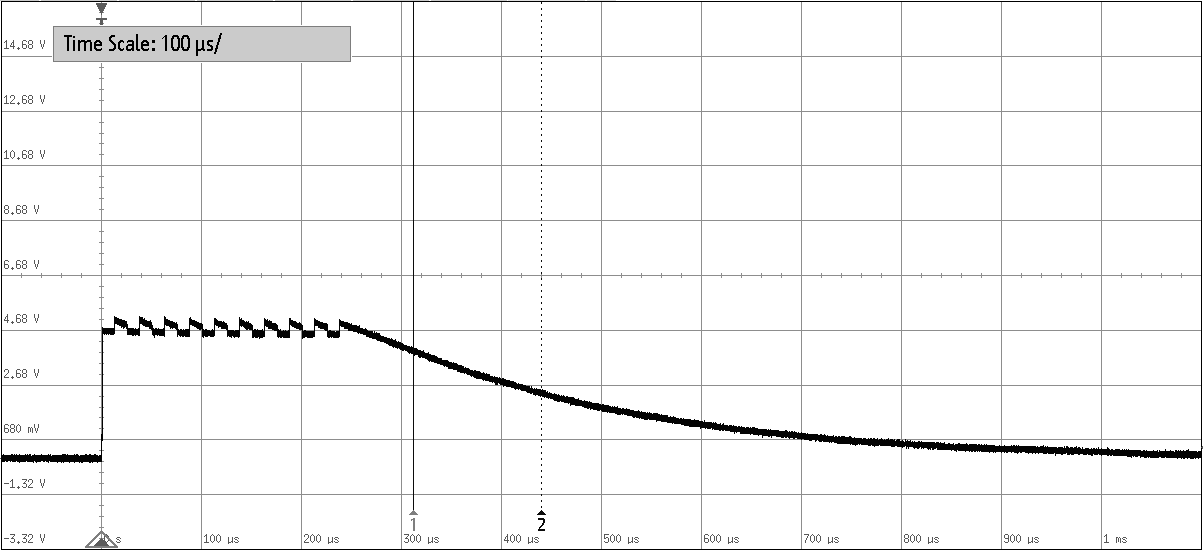
\includegraphics[width=1\textwidth%, draft
]{Abbildungen/MessungenP1/PWM-ausgabe-mit-Hi-Side.png}
\captionof{figure}{PWM Ausgabe über einen Hi-Side}
\label{fig:HiSide}
\end{minipage}
In der Abbildung \ref{fig:pwm-burst} ist zu sehen, dass ein Burst aus zehn Impulsen mit einer Periodendauer von jeweils 25us vom Mikrocontroller generiert wurde. Diese Messung wurde auch vorgenommen, um zu überprüfen, wie sich das Signal durch die eingesetzten Bauteile verändert.\\
Die Abbildung \ref{fig:HiSide} zeigt, wie das Ausgangssignal nach einer Hi-Side aussieht. So wird zwar im Takt des PWM-Signals geschaltet, allerdings fehlt es an einem Gegenpool, um das Potential in den Schaltpausen wieder auf Null zu ziehen. Dadurch bleibt die Spannung während des Schaltens immer auf einem erhöhten Pegel und sinkt erst nach Ende des PWM-Signals langsam ab. Dadurch kann natürlich keine vernünftige Ausgabe am Lautsprecher erzeugt werden, denn ohne deutliche Potentialunterschiede kann dieser auch nicht in Schwingungen versetzt werden. Der ausgegebene Schalldruck würde maximal für kürzeste Entfernungsmessungen reichen, wenn überhaupt und dann würde das zurückkommende Signal noch von der abklingenden Spannung des Hi-Side überlagert. Dadurch ist dieser Aufbau nicht operabel.\\Um die Spannung sauber auf Hi- und LOW-Pegel schalten zu können wurde somit auf eine Halbbrücke gewechselt. Bei der ersten, einfach gesteuerten Version, entstand das Problem, dass beim Schalten der Halbbrücke, in den Schaltmomenten, Kurzschlüsse entstanden, weil beide MOSFETs gelichzeitig geschaltet haben. Somit wurde auf eine voll gesteuerte Halbbrücke gewechselt und es wurden zwei PWM-Signale moduliert, bei denen eines invertiert und die Flanken derart verschoben waren, dass die angesteuerten MOSFETs nie Kurzschlüsse schalten können. Mit der verwendeten, vollgesteuerten Halbbrücke ergab sich die Abbildung \ref{fig:Halfbridge}\\
\begin{minipage}{0.5\textwidth}
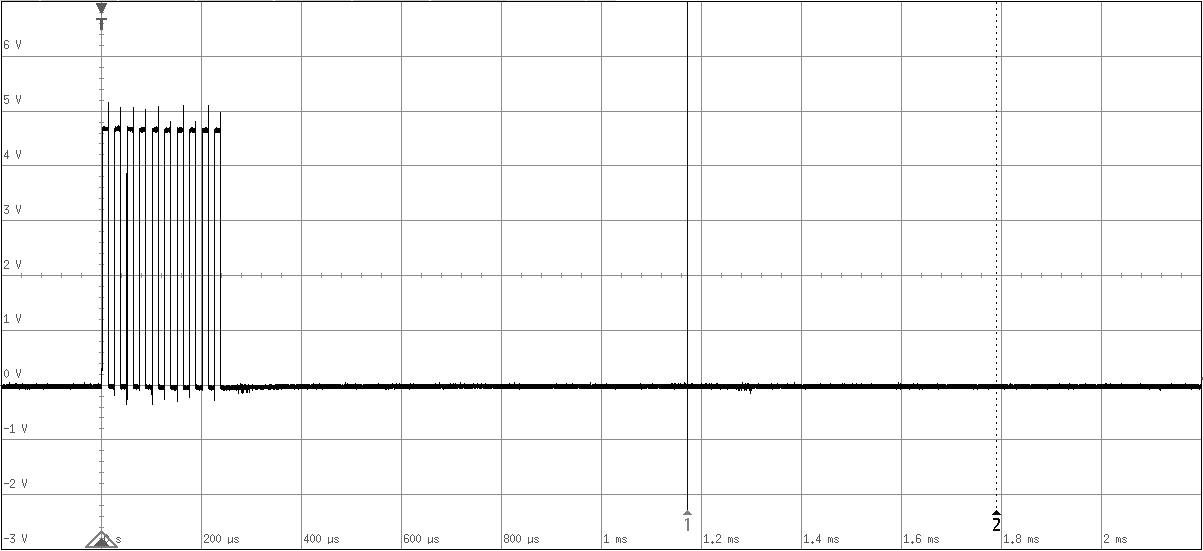
\includegraphics[width=1\textwidth%, draft
]{Abbildungen/MessungenP1/PWM-Nach-der-Halbbrucke.png}
\captionof{figure}{PWM Ausgabe über eine Halbbrucke}
\label{fig:Halfbridge}
\end{minipage}
\begin{minipage}{0.5\textwidth}
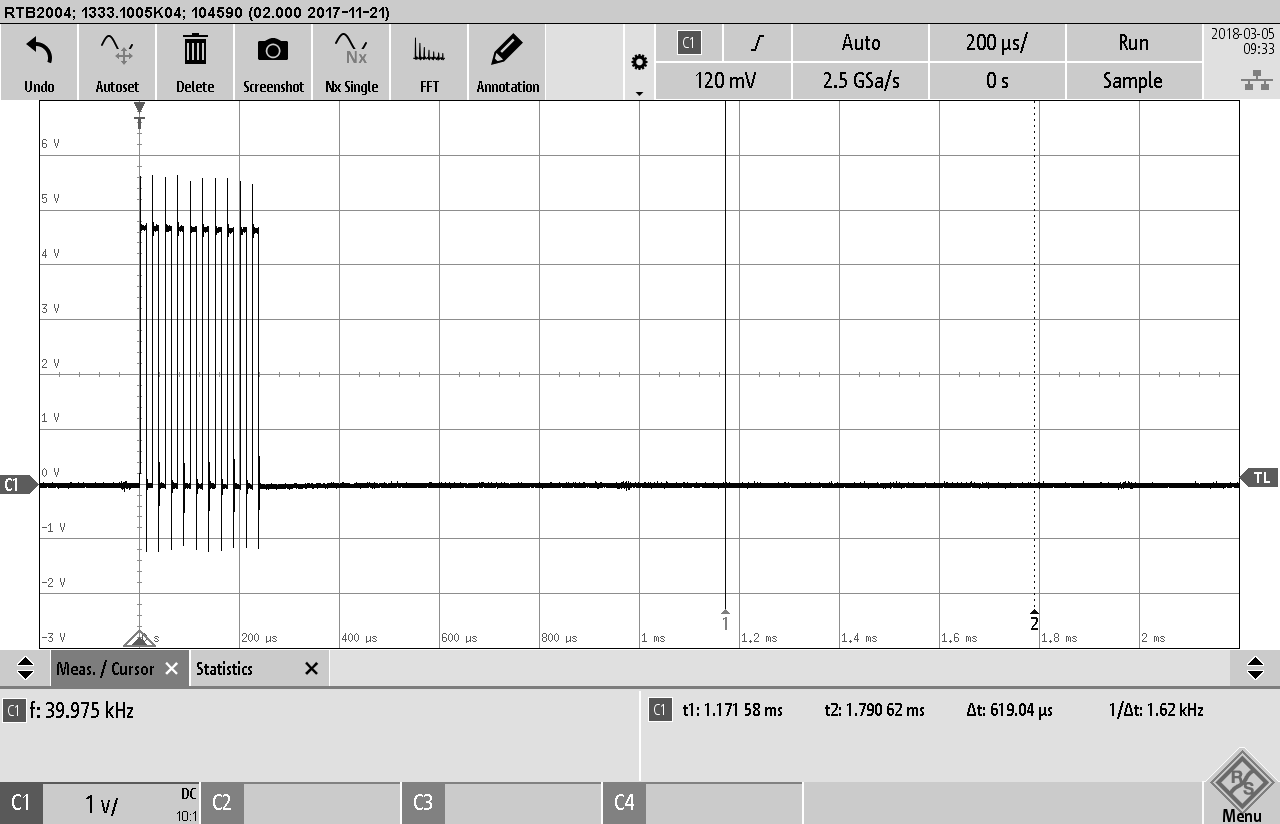
\includegraphics[width=1\textwidth%, draft
]{Abbildungen/MessungenP1/PWM-Nach-der-Halbbrucke-mit-LS.png}
\captionof{figure}{Ausgabe der PWM mit erhöhter Amplitude am Sender}
\label{fig:Sender}
\end{minipage}
Es zeigt sich, dass das Signal nach der Erweiterung auf eine Halbbrücke wieder wie das von der CPU ausgegebene PWM-Signal \ref{fig:pwm-burst} aussieht, nur dass die Amplitude wie geplant höher ausfällt. Somit kann die Höhe der Amplitude über die Spannungspumpe variiert werden um die Stärke des ausgegebenen Signals zu variieren, ohne die CPU durch die höhere Spannung zu beschädigen.
Wie in der Abbildung \ref{fig:Sender} zu entnehmen ist, entstehen durch die angeschlossene Ultraschallkapsel höhere Spannungsimpulse im Einschaltmoment.

\subsection{Empfängerkreis}
Der auf einer zweiten Platine aufgebaute Empfängerkreis wurde getrennt vom Senderkreis getestet, um eine mögliche Überlagerung der elektrischen Signale zu verhindern. Dafür wurden beide Platinen auf einem Versuchsaufbau befestigt und die Sender- und die Empfängerkapsel nebeneinander, parallel ausgerichtet, befestigt.\\
\begin{minipage}{0.5\textwidth}
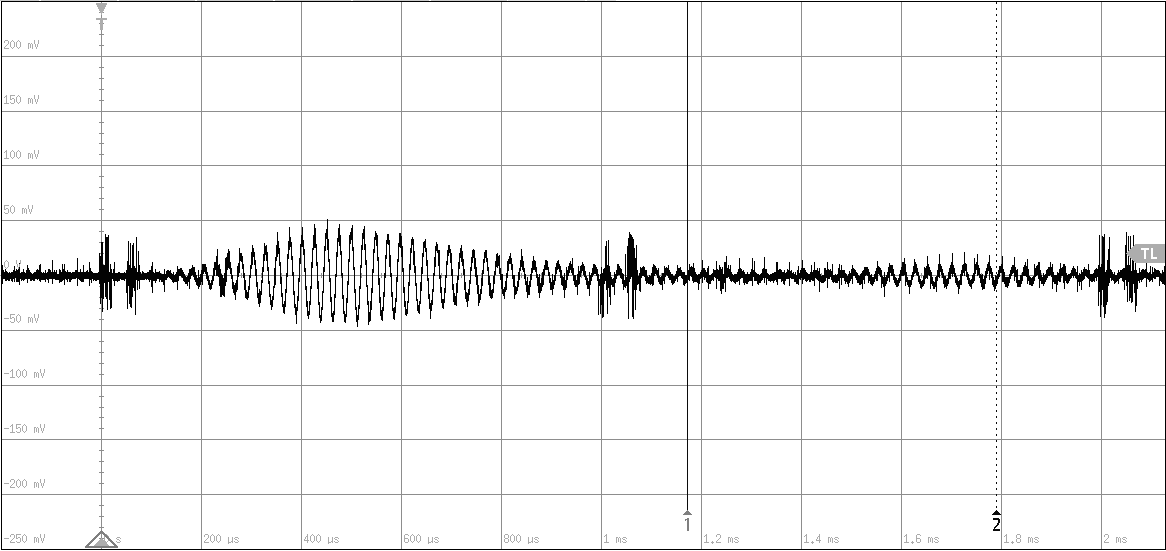
\includegraphics[width=1\textwidth%, draft
]{Abbildungen/MessungenP1/Signal-Empfang.png}
\captionof{figure}{Signal Empfang}
\label{fig:Empfang am LS}
\end{minipage}
\begin{minipage}{0.5\textwidth}
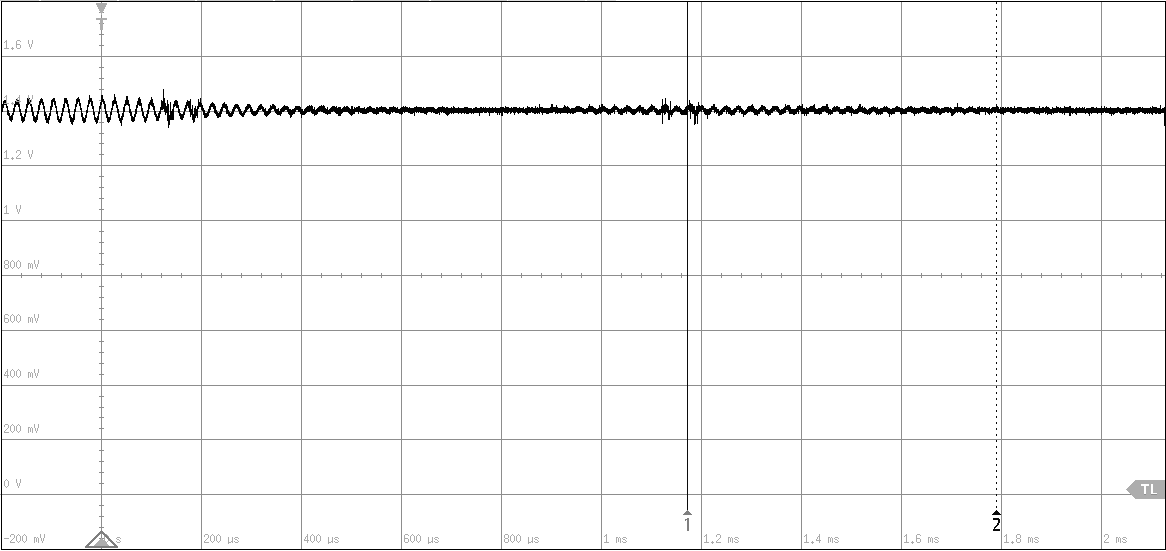
\includegraphics[width=1\textwidth%, draft
]{Abbildungen/MessungenP1/Signal-nach-der-Filterung.png}
\captionof{figure}{Signal nach der Filterung}
\label{fig:Filterung}
\end{minipage}
Die Abbildung \ref{fig:Empfang am LS} zeigt das Signal, das direkt am Empfänger zu messen war. Hier sind verschiedene vorerst nicht zuordnenbare Signale zu sehen. Allein aus diesem Bild lässt sich aber keine Aussage zu den Signalen machen, fest steht nur dass ebenfalls Signale, die nicht der gewünschten Frequenz entsprechen ebenfalls vom Empfänger aufgenommen werden. Diese gilt es natürlich schnellst möglich auszumerzen, um unerwünschte Störungen zu vermeiden.
In der Abbildung \ref{fig:Filterung} ist das Signal nach dem eingebauten Hochpassfilter zu sehen.\\
\begin{minipage}{0.5\textwidth}
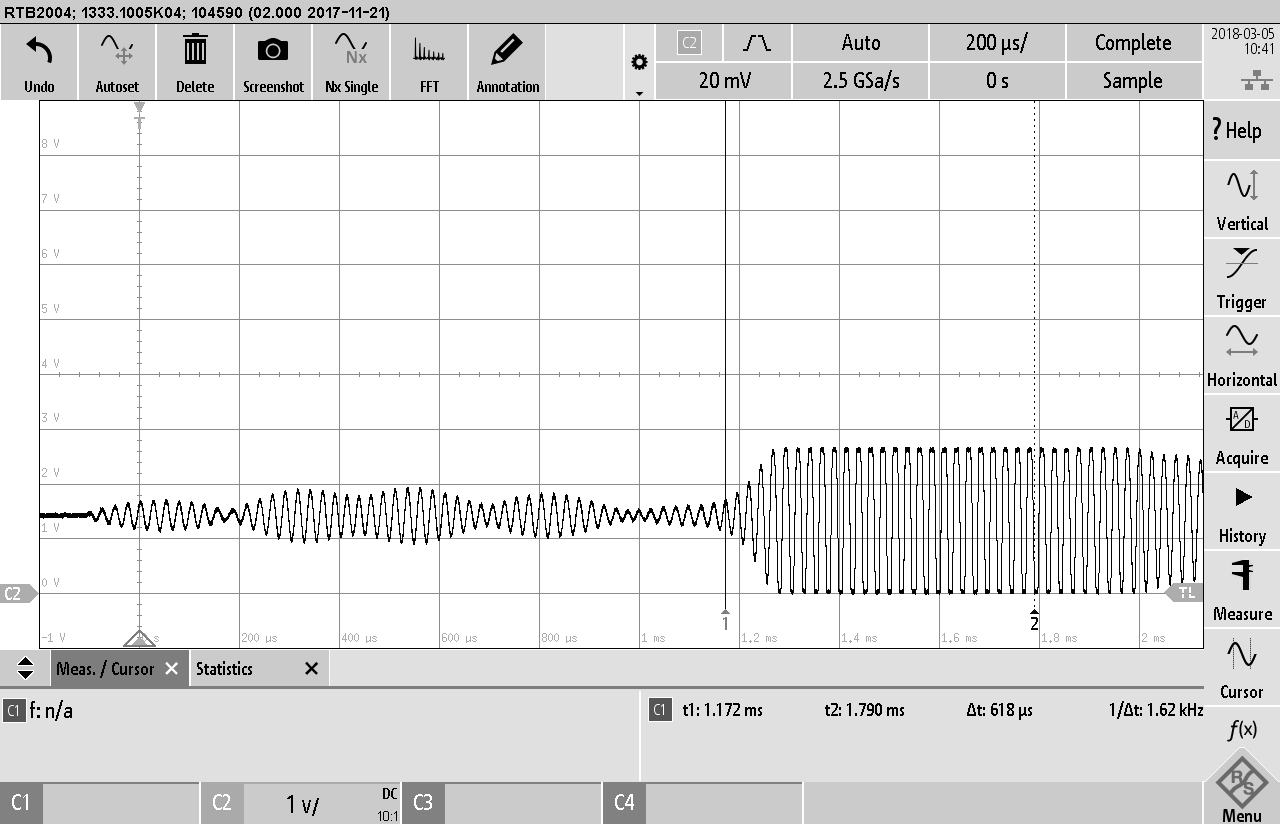
\includegraphics[width=1\textwidth%, draft
]{Abbildungen/MessungenP1/Signal-nach-Verstarkung.png}
\captionof{figure}{Signal nach Verstärkung}
\label{fig:Verstaerkung}
\end{minipage}
\begin{minipage}{0.5\textwidth}
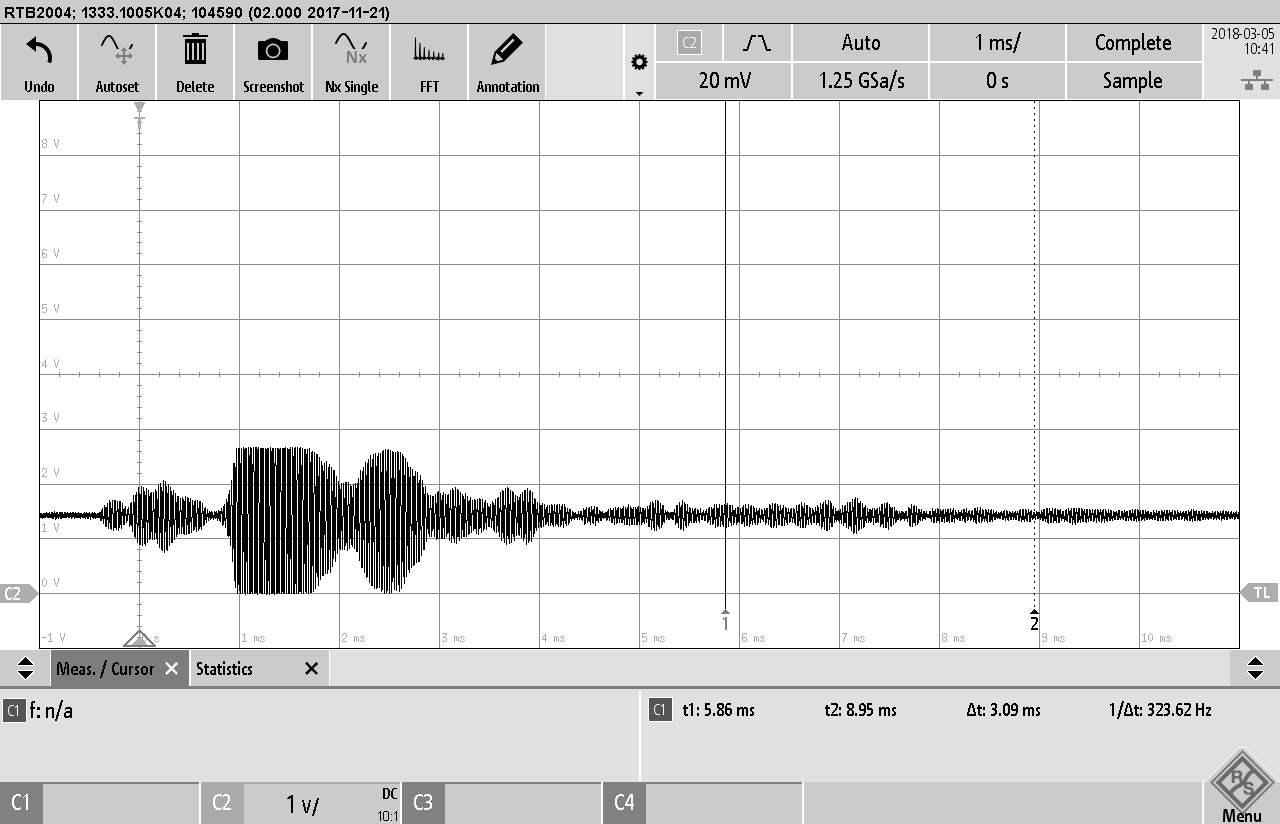
\includegraphics[width=1\textwidth%, draft
]{Abbildungen/MessungenP1/Signal-nach-Verstarkung2.png}
\captionof{figure}{Signal nach Verstärkung2}
\label{fig:Verstaerkung2}
\end{minipage}
Der erste Operationsverstärker dient der Verstärkung des gefilterten Eingangssignals. Dieses ist notwendig, da das ausgesendete Schallsignal mit zunehmendem Weg an Schalldruck verliert, und beim Eintreffen am Empfänger deutlich niedrigere Spannungen erzeugt, als beim absenden eingesetzt wurden. \\
\begin{minipage}{0.5\textwidth}
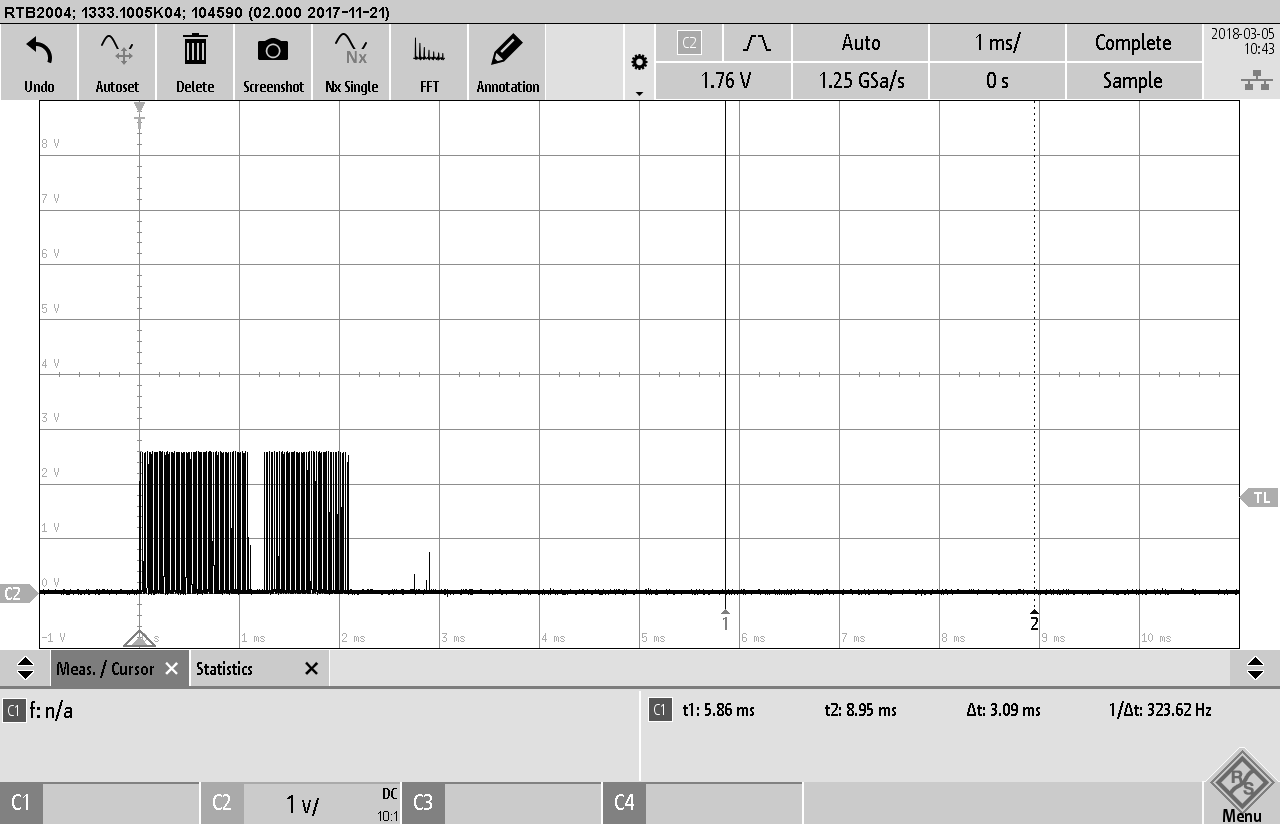
\includegraphics[width=1\textwidth%, draft
]{Abbildungen/MessungenP1/Signal-nach-Komparator.png}
\captionof{figure}{Signal nach Komparator}
\label{fig:Komparator}
\end{minipage}\\
Nach dem das Signal den Komparator passiert hat, ergibt sich das Bild wie in Abbildung \ref{fig:Komparator} zu sehen ist. Aus dem anfänglichen Eingangssignal, aus dem nichts verwertbares abzulesen war, ist ein wesentlich übersichtlicheres Signal entstanden. Nun sind lediglich zwei Signalblöcke übriggeblieben, die beide eine Frequenz von 40kHz haben. Bei dem ersten Signalblock handelt es sich um ein Störsignal, denn es ist das vom Sender ausgesandte Signal, das seitlich auf den Empfänger abstrahlt. Der zweite Signalblock ist dagegen das Echo, also das Signal, das vom Hindernis zurückgeworfen wurde. Mit diesem Signal ließe sich die Entfernung zum Hindernis berechnen.\\
Nachfolgend wurden die Signalverläufe mit verschiedenen Ultraschallkapseln aufgenommen, um vergleichen zu können, wie die Signalqualität bei verschiedenen Produkten schwankt. Dabei wurde die Amplitude von 4,6V für das Sendersignal und die Verstärkung des Empfängers auf ein Minimum eingestellt.\\
\begin{minipage}{0.5\textwidth}
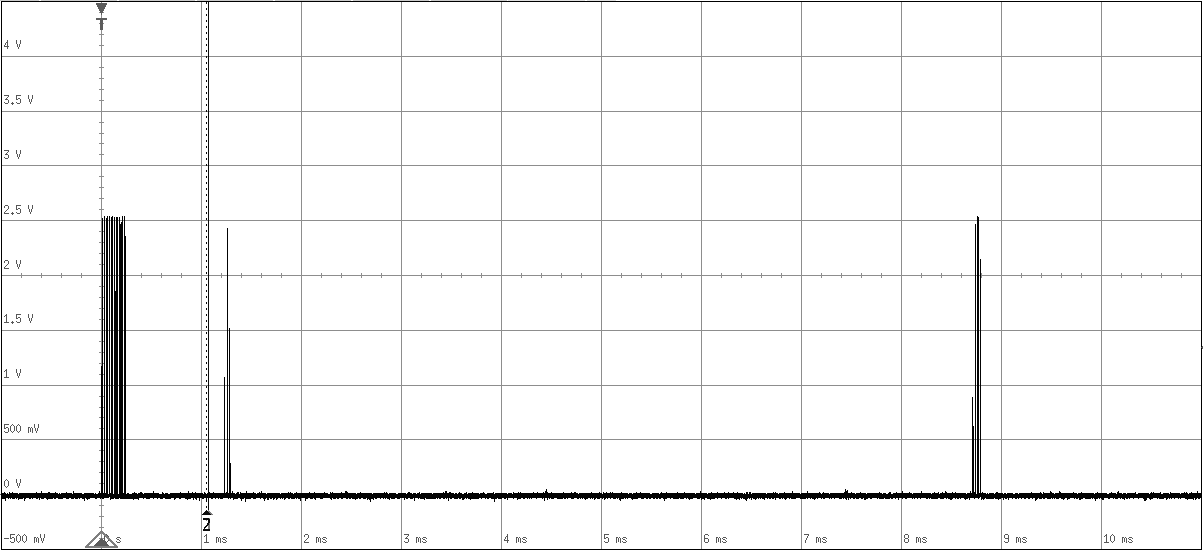
\includegraphics[width=1\textwidth%, draft
]{Abbildungen/MessungenP1/EKULIT1,5m.png}
\captionof{figure}{EKULIT 1,5m}
\label{fig:EKULIT1,5m}
\end{minipage}
\begin{minipage}{0.5\textwidth}
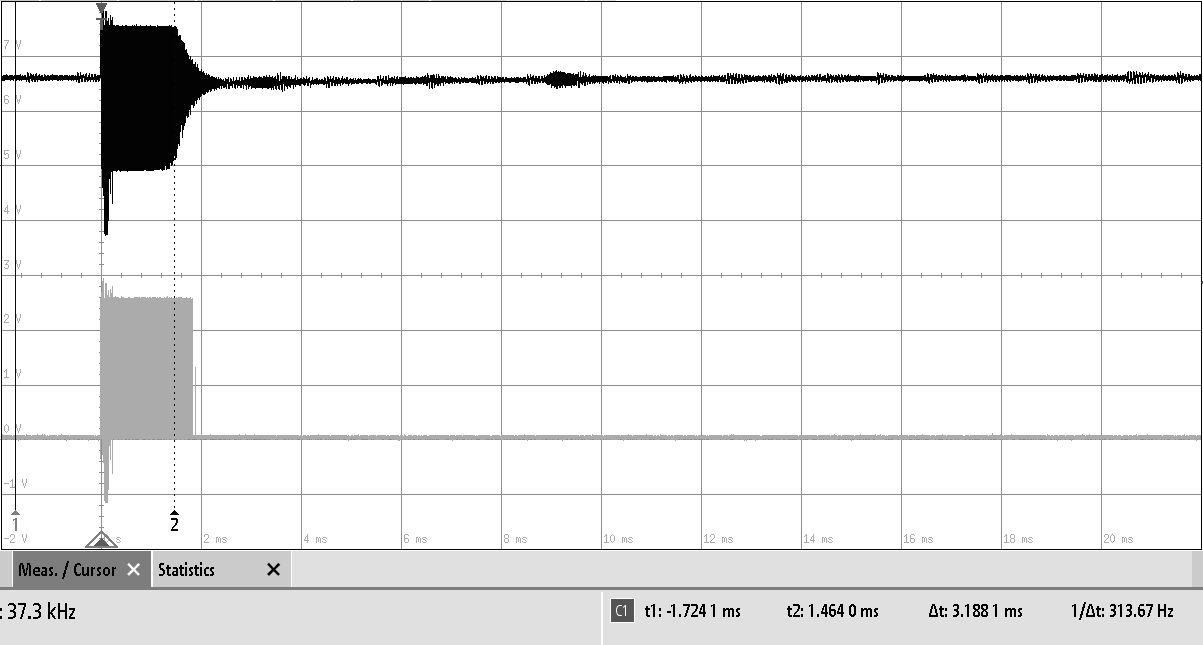
\includegraphics[width=1\textwidth%, draft
]{Abbildungen/MessungenP1/MURATAr1,5m.png}
\captionof{figure}{MURATA reciver 1,5m}
\label{fig:MURATA reciver 1,5m}
\end{minipage}
\begin{minipage}{0.5\textwidth}
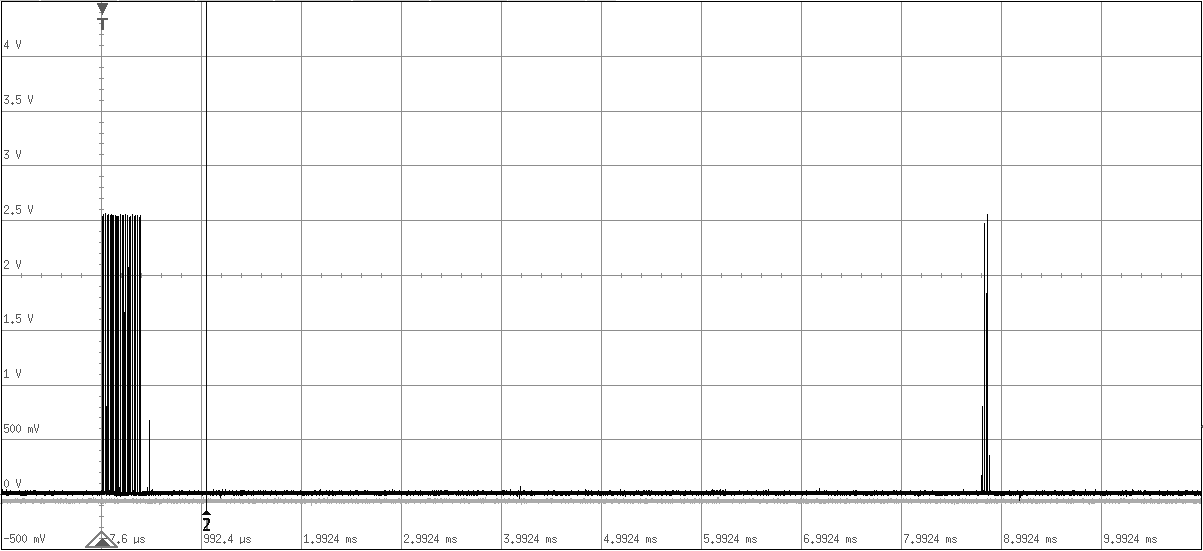
\includegraphics[width=1\textwidth%, draft
]{Abbildungen/MessungenP1/MURATAs1,5m.png}
\captionof{figure}{MURATA sender 1,5m}
\label{fig:MURATA sender 1,5m}
\end{minipage}
\begin{minipage}{0.5\textwidth}
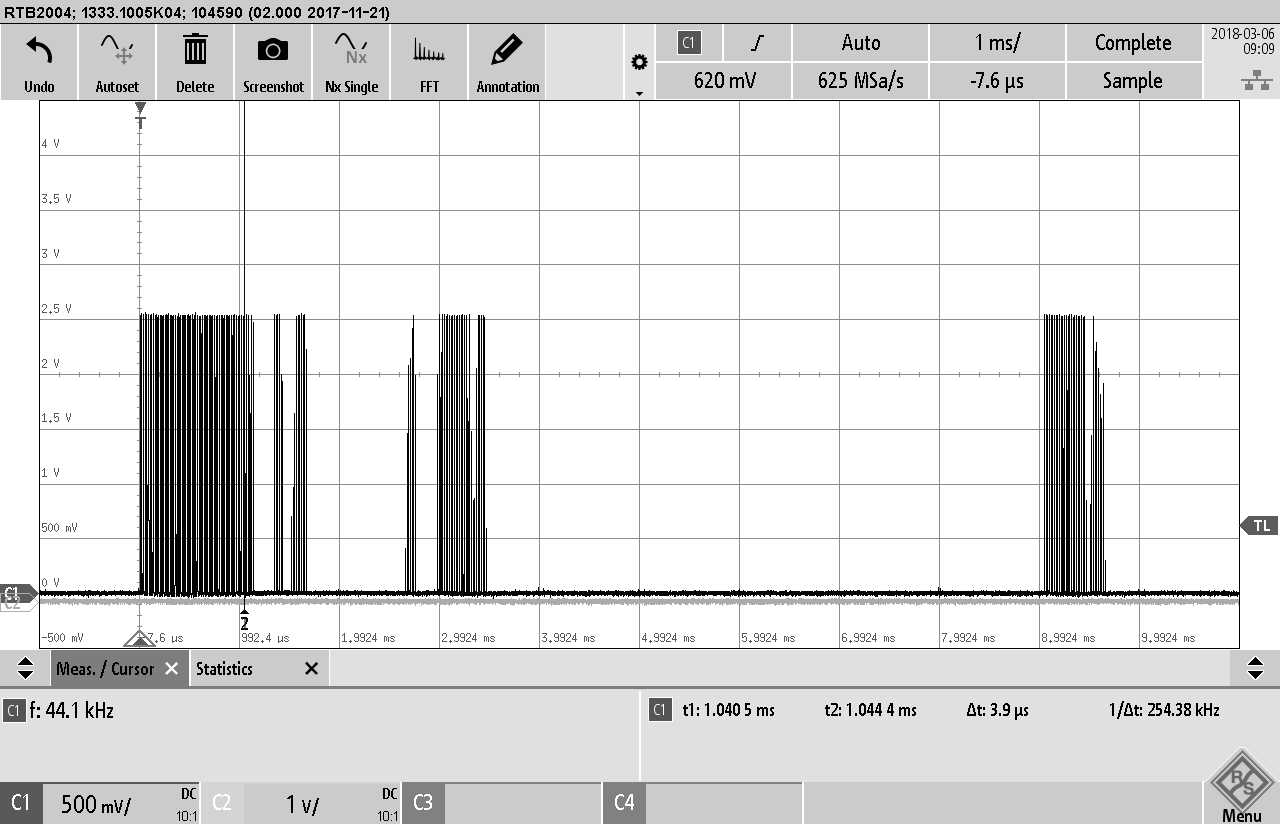
\includegraphics[width=1\textwidth%, draft
]{Abbildungen/MessungenP1/MURATAsr1,5m.png}
\captionof{figure}{MURATA sender + reciver 1,5m}
\label{fig:MURATA sender+reciver}
\end{minipage}\\
Bei den Ultraschallkapseln von EKULIT zeigte sowohl eine Verpoolung der Anschlüsse, als auch ein Tausch von Sender- und Empfängerkapsel keinen Unterschied. Bei den Ultraschallkapseln von MURATA sind bei der Wahl der Kapseln dagegen deutliche Unterschiede zu sehen. Werden nur die Sender-Kapseln als Sender und Empfänger verwendet, entsteht das in Abbildung \ref{fig:MURATA sender 1,5m} zu sehende Signal. Die Breite des eingehenden Echo Signals ist deutlich geringer, als bei den anderen verwendeten Kombinationen. Am besten sind die Signale bei der Kombination aus Sender und Empfänger von MURATA, Abbildung \ref{fig:MURATA sender+reciver} oder bei den EKULIT-Kapseln, Abbildung \ref{fig:EKULIT1,5m}.

\section{Prototyp 2}

Bei einer Betrachtung der Signalverläufe einer Entfernungsmessung, ließen sich die folgenden Signale aufnehmen. Die Spannung von der Spannungspumpe wurde auf 10v eingestellt, zu sehen sind die Signalverläufe nach dem Verstärker und nach dem Komparator.\\
\begin{minipage}{0.5\textwidth}
\includegraphics[width=1\textwidth%, draft
]{Abbildungen/MessungenP2/10V/EKULIT1m.png}
\captionof{figure}{Signalverlauf bei 10V auf 1m Abstand}
\label{fig:EKULIT 1m}
\end{minipage}
\begin{minipage}{0.5\textwidth}
\includegraphics[width=1\textwidth%, draft
]{Abbildungen/MessungenP2/10V/EKULIT2m.png}
\captionof{figure}{Signalverlauf bei 10V auf 2m Abstand}
\label{fig:EKULIT 2m}
\end{minipage}
\begin{minipage}{0.5\textwidth}
\includegraphics[width=1\textwidth%, draft
]{Abbildungen/MessungenP2/10V/EKULIT3m.png}
\captionof{figure}{Signalverlauf bei 10V auf 3m Abstand}
\label{fig:EKULIT 3m}
\end{minipage}\\
In den Abbildungen sind jeweils zwei PWM-Ausgaben und die darauf folgenden Echos zu sehen. So trifft das Echo in Abbildung \ref{fig:EKULIT 1m} etwa 6,ms nach dem absenden des ersten Impulses  wieder an der Ultraschallkapsel ein. In der Abbildung \ref{fig:EKULIT 3m} ist das Echo so schwach, dass die Verstärkung bereits nicht mehr ausreicht, um noch ein Signal nach dem Komparator zu ermöglichen.\\
Bei einer Erhöhung der Spannung von der Spannungspumpe auf einen Wert von 15,75V (Spitzenwerte an der Ultraschallkapsel von 20V) sind die nachfolgenden Signalverläufe entstanden.\\
\begin{minipage}{0.5\textwidth}
\includegraphics[width=1\textwidth%, draft
]{Abbildungen/MessungenP2/15,75V/EKULIT1m.png}
\captionof{figure}{Signalverlauf bei 15,75V auf 1m Abstand}
\label{fig:EKULIT2 1m}
\end{minipage}
\begin{minipage}{0.5\textwidth}
\includegraphics[width=1\textwidth%, draft
]{Abbildungen/MessungenP2/15,75V/EKULIT2m.png}
\captionof{figure}{Signalverlauf bei 15,75V auf 2m Abstand}
\label{fig:EKULIT2 2m}
\end{minipage}
\begin{minipage}{0.5\textwidth}
\includegraphics[width=1\textwidth%, draft
]{Abbildungen/MessungenP2/15,75V/EKULIT3m.png}
\captionof{figure}{Signalverlauf bei 15,75V auf 3m Abstand}
\label{fig:EKULIT2 3m}
\end{minipage}\\
In den obigen Abbildungen ist zu sehen, dass die Signalstärke der Echos durch die Erhöhung der Spannung leicht zugenommen hat. Gerade bei einem Vergleich der Abbildungen \ref{fig:EKULIT 3m} und \ref{fig:EKULIT2 3m} ist zu sehen, dass der Komparator durch die Signalerhöhung auch bei dem Echo das Schalten beginnt. Das heißt, dass bereits durch die Signalstärke am Sender ein Betrieb bis 3m Abstand möglich ist.




























